\chapter{Эллиптический бильярд с косинусным законом преломления на софокусных квадриках.}\label{ch:ch3}

\section{Введение.}\label{sec:ch3/sect1}
Интерес к составным бильярдам возникает в связи с активно разрабатываемой  в школе А.~Т.~Фоменко теорией бильярдов со сложной топологией, таких как бильярдные книжки. Современное состояние этой теории см. в обзоре [1].  

Рассмотрим ограниченную эллипсом область, разбитую дугой софокусной квадрики на две области с разными плотностями, но постоянными внутри каждой из областей. Тогда мы можем рассмотреть бильярдную траекторию, которая при пересечении границы раздела двух сред меняет направление по закону Снеллиуса [2]: отношение синусов углов падения и преломления равно обратному отношению плотностей сред. 
Экспериментальная компьютерная проверка демонстрирует, что такой бильярд неинтегрируем. 

С другой стороны, в физике известны законы преломления другого вида. 
В задачах теплопроводности направление векторов плотностей теплового потока на границе раздела двух сред определяется отношением тангенсов [3, 4].
В некоторых задачах оптики встречаются законы, формулируемые в терминах отношения косинусов углов падения и преломления [5, 6].

В настоящей работе мы рассматриваем бильярд в эллипсе, разделенном дугами софокусных квадрик на несколько областей $\Omega_i$ с постоянными в них плотностями $n_i$, при этом закон преломления задан равенством $n_1 \cos{\theta_1} = n_2 \cos{\theta_2}$. Мы покажем, что в полученная система будет интегрируемой (см. пункты 5 и 6) и предъявим дополнительный интеграл. В некоторых случаях значения этого дополнительного интеграла принадлежат не прямой, а окружности, см. пункт 7.


\section{Классический бильярд.}

Зафиксируем большую и малую полуоси эллипса $a$ и $b$, где $a > b > 0$ и во внутренности эллипса $\left(f(x, y) = \dfrac{x^2}{a^2}+\dfrac{y^2}{b^2} < 1 \right)$ рассмотрим движение материальной точки с координатами $\mathbf{x} = (x, y)$ и вектором скорости $\mathbf{v} = (v_x, v_y)$, при котором на границе эллипса $f(x, y) = 1$ векторы скорости до отражения и после него образуют равные по величине углы с вектором нормали $n=\left.\nabla f(x,y)\right|_{(x_0,y_0)} = \left( \dfrac{2x_0}{a^2},\dfrac{2y_0}{b^2}\right)$ к эллипсу в точке отражения $(x_0, y_0)$.

Обозначим $\Psi = \left\{ Q_{\lambda} \ |\ \lambda \in (0, a^2) \right\}$ -- однопараметрическое семейство софокусных квадрик, где квадрика $Q_\lambda$ задается уравнением 
$f_\lambda(x,y)=\dfrac{x^2}{a^2-\lambda} + \dfrac{y^2}{b^2-\lambda} = 1$.

Интегрируемость классического бильярда обусловлена классической теоремой из геометрии: если какое-то звено бильярдной траектории коснулось софокусной квадрики $Q_\lambda$ из семейства $\Psi$, то и все остальные звенья касаются этой же квадрики, поэтому $\lambda$ является первым интегралом.


\section{Интеграл Иоахимсталя.}\label{sec:ch3/formatted-numbers}
Пусть $M = Q_0 \times \mathbb{R}^2$ -- фазовый цилиндр бильярда в эллипсе $Q_0$. Для точки $(\mathbf{x}, \mathbf{v}) = ((x,y), (v_x, v_y)) \in M$ рассмотрим функцию $J(\mathbf{x}, \mathbf{v}) = -\left(
\frac{x v_x}{a^2} + \frac{y v_y}{b^2} \right).$
Функция $J(\mathbf{x}, \mathbf{v})$ не является интегралом движения точки в эллиптическом бильярде, так как не сохраняется на прямолинейных отрезках траектории. Тем не менее, для <<дискретного>> бильярда в эллипсе, когда траектория записывается последовательностью точек на эллипсе, в которых траектории испытывают отражения, функция $J(\mathbf{x}, \mathbf{v})$ является интегралом. А именно, прямолинейное звено бильярдной траектории будем кодировать начальной точкой звена $(x, y)$ и его вектором скорости $(v_x, v_y)$. Тогда выполняется следующее утверждение: 

\begin{theorem}{\normalfont{[7, с.~61]}}.
Пусть $(\mathbf{x}_i, \mathbf{v}_i) \in M, \quad i=1,\ldots$, -- последовательность точек на фазовом цилиндре, кодирующая последовательные звенья некоторой  бильярдной траектории. Тогда $J(\mathbf{x}_i, \mathbf{v}_i) =  J(\mathbf{x}_{i+1}, \mathbf{v}_{i+1})$ для всех $i$.
\label{th:sect3_th1}
\end{theorem}

Функцию $J$ называют интегралом Иоахимсталя. Заметим, что эту функцию можно переписать в виде 
$$J(\mathbf{x}, \mathbf{v}) = -\frac{1}{2}\langle\mathbf{v}, \nabla f_0(x, y)\rangle,$$
где $\langle\cdot, \cdot\rangle$ обозначает скалярное произведение. 

Прежде чем перейти к геометрическому смыслу интеграла Иоахимсталя, рассмотрим следующий вопрос: сколько квадрик из семейства $\Psi = \left\{ Q_{\lambda} \ |\ \lambda \in (0, a^2) \right\}$ касаются   фиксированной произвольным образом прямой в $\mathbb{R}^2$?

\begin{statement}
Рассмотрим прямую $\mathbf{x}+t\mathbf{v}$, проходящую через точку $\mathbf{x}= (x, y)$ на плоскости $\mathbb{R}^2$ и имеющую направление $\mathbf{v}=(v_x, v_y)$. Тогда:

$(i)$ Прямая касается не более одной квадрики $Q_\lambda$ из семейства $\Psi$.

$(ii)$ Исключая вертикальную ось $x=0$ и прямые, проходящие хотя бы через один из фокусов,  такая касательная квадрика  $Q_\lambda$ существует и ее параметр $\lambda$ определяется по формуле 
\begin{equation}
\lambda = \Lambda(\mathbf{x}, \mathbf{v}) = \frac{a^2 v_y^2 + b^2v_x^2 - (x v_y-y v_x)^2}{v_x^2 + v_y^2}.
\label{eq:sect3_eq1}
\end{equation}

\end{statement}

\begin{proof}
Прямая $\mathbf{x} + t \mathbf{v}$ касается квадрики $Q_\lambda$ тогда и только тогда, когда уравнение
$$\frac{(x + t v_x)^2}{a^2-\lambda} + \frac{(y + t v_y)^2}{b^2-\lambda} = 1$$
имеет ровно одно решение по $t$, то есть когда дискриминант квадратного уравнения с переменной $t$  равен нулю. Приравнивая дискриминант к нулю и решая равенство относительно параметра софокусной квадрики $\lambda$ можно получить формулу \eqref{eq:sect3_eq1} из второго пункта формулировки утверждения. В случаях, если $\lambda = a^2$ или $\lambda = b^2$, касательная квадрика $Q_\lambda$ вырождается в прямую (проходящую через малую полуось при $\lambda = a^2$ и проходящая через большую полуось при $\lambda = b^2$), следовательно прямая $\mathbf{x}+ t\mathbf{v}$ не касается никакой софокусной квадрики $Q_\lambda$.
\end{proof}

Заметим, что для бильярда в эллипсе вычисленный в точке $(\mathbf{x}, \mathbf{v})$ фазового цилиндра $M$ интеграл Иоахимсталя связан с параметром софокусной квадрики $\lambda$, которой касается прямая с направляющим вектором $\mathbf{v}$, проходящая через точку $\mathbf{x}$.

\begin{statement}
    Пусть $(\mathbf{x}, \mathbf{v})$ кодируют некоторое звено бильярдной траектории. Пусть $\lambda$ -- параметр квадрики $Q_\lambda$, касающейся прямой $\mathbf{x} +t \mathbf{v}$. Тогда 
    \begin{equation}
        \lambda = \Lambda(\mathbf{x}, \mathbf{v}) =  a^2 b^2 \frac{J^2(\mathbf{x}, \mathbf{v})}{||\mathbf{v}||^2}
    \label{eq:sect3_eq2}
    \end{equation}
\end{statement}

\begin{proof}
Выражение \eqref{eq:sect3_eq1} для $\lambda$ перепишем, домножив обе части на знаменатель:
\begin{equation}
(v_x^2 + v_y^2)\lambda = a^2 v_y^2 + b^2v_x^2 - (x v_y-y v_x)^2 = (a^2-x^2)v_y^2 + (b^2-y^2)v_x^2 + 2 x y v_x v_y.
\label{eq:sect3_eq3}
\end{equation}
Точка $(x, y)$ находится на эллипсе $Q_0$, поэтому
\begin{equation}
a^2 - x^2 = \frac{a^2 y^2}{b^2} \text{  и } b^2 - y^2 = \frac{b^2 x^2}{a^2}.
\label{eq:sect3_eq4}
\end{equation}
Подставляя \eqref{eq:sect3_eq4} в \eqref{eq:sect3_eq3}, получаем
$$||\mathbf{v}||^2 \lambda = \frac{a^2y^2}{b^2} + \frac{b^2 x^2}{a^2} + 2 x y v_x v_y = ||\mathbf{v}||^2 a^2b^2 \left( \frac{x v_x}{a^2} + \frac{y v_y}{b^2}\right)^2 = a^2b^2J^2(\mathbf{x}, \mathbf{v}).$$
\end{proof}

\section{Классический бильярд.}
Предположим, что две среды с показателями <<плотности>> $n_1$ и $n_2$ разделены кривой $Q_0$. Пусть падающая траектория из среды с показателем $n_1$ пересекает $Q_0$ в некоторой точке. Будем считать, что при $n_1 \cos \theta_1 < n_2$  преломленная траектория из этой точки уходит в область с показателем преломления $n_2$ и в другую полуплоскость по отношению к вектору нормали $\mathbf{n}$, причем выполняется  закон преломления 
 \begin{equation}
n_1 \cos{\theta_1} = n_2 \cos{\theta_2},
\label{eq:sect3_eq5}
\end{equation}
где $\theta_1, \theta_2$ --- углы, образованные падающим и преломленным отрезками траектории, соответственно, по отношению к вектору нормали $\mathbf{n}$ к кривой $Q_0$ в точке преломления.

Если $n_1 > n_2$ и $\cos \theta_1 > \dfrac{n_2}{n_1}$, тогда угол $\theta_2$ не определен и мы считаем, что траектория испытывает полное внутреннее отражение по классическому закону <<угол падения равен углу отражения>>. 

Если же $\dfrac{n_1}{n_2} < 1 $ и $\cos \theta_1 = 1$, тогда  $\theta_2 = \arccos \dfrac{n_1}{n_2}$, и существуют два способа определить вектор скорости после преломления: 
\begin{equation}
    \mathbf{w}= \left[
\begin{array}{rr}
    R(\theta_2) \mathbf{v}, & \text{<<левая траектория>>} \\
    R(-\theta_2) \mathbf{v},  & \quad \text{<<правая траектория>>}
\end{array}
\right.,
\label{eq:sect3_eq6}
\end{equation}
где $R(\phi) = 
\left(
    \begin{array}{rr}
    \cos \phi \ & -\sin \phi \\
    \sin \phi \ & \cos \phi 
    \end{array}
\right)
    $ --- матрица поворота.
Мы будем считать, что в такой ситуации <<левая>> или <<правая>> траектории выбираются случайно. Ниже будет показано, что в случае, который рассматривается в настоящей статье, значение дополнительного интеграла в обоих случаях будет одно и то же, т.е. этот случайный выбор на интегрируемости не сказывается.


Для простоты будем считать, что модуль вектора скорости при преломлении или полном отражении не меняется; тогда кинетическая энергия $E=\dfrac{m || \mathbf{v} || ^2}{2} $ постоянна на траекториях.

 \begin{statement}
Пусть $\mathbf{n}$ -- вектор нормали в точке преломления $(x_0, y_0)$, а также пусть $\mathbf{v}$ -- вектор скорости до преломления. Считаем, что траектория бильярда в точке $(x_0, y_0)$ переходит из среды с показателем преломления $n_1$ в область с показателем $n_2$. Тогда если вектор $\mathbf{v}$ не параллелен вектору $\mathbf{n}$, то для вектора   $\mathbf{w}$  после преломления справедливо выражение 
$\mathbf{w} = \alpha \mathbf{v} + \beta \mathbf{n}$, где $\beta = \dfrac{||\mathbf{w}|| \mu - ||\mathbf{v}|| \alpha}{||\mathbf{n}||}\cos{\theta_1}$, $\alpha = \dfrac{||\mathbf{w}||}{||\mathbf{v}||}\sqrt{\dfrac{1-\mu^2\cos^2 \theta_1}{1-\cos^2 \theta_1 }}$, $\theta_1$ -- угол, образованный векторами $\mathbf{v}$ и $\mathbf{n}$, $\mu = \dfrac{n_1}{n_2}$.
\end{statement}
\begin{proof}
Из закона преломления \eqref{eq:sect3_eq5} следует 
$\langle\mathbf{w}, \mathbf{n}\rangle = ||\mathbf{w}||\, ||\mathbf{n}|| \cos \theta_2 = ||\mathbf{w}||\, ||\mathbf{n}|| \mu \cos \theta_1$.

В то же время, из линейности скалярного произведения
$\langle\mathbf{w}, \mathbf{n}\rangle = \alpha \langle\mathbf{v}, \mathbf{n}\rangle + \beta\, ||\mathbf{n}||^2 = \alpha ||\mathbf{v}||\, ||\mathbf{n}|| \cos \theta_1 + \beta\, ||\mathbf{n}||^2$, следовательно, $\beta = \dfrac{||\mathbf{w}|| \mu - ||\mathbf{v}|| \alpha}{||\mathbf{n}||}\cos{\theta_1}$. 

Подставляя полученное значение $\beta$ в равенство $||\mathbf{w}||^2 = ||\alpha \mathbf{v} + \beta \mathbf{n}||^2 = \alpha^2 ||\mathbf{v}||^2 (1-\cos^2 \theta_1) + \mu^2||\mathbf{w}||^2 \cos^2 \theta_1$, получим нужную формулу для  $\alpha$.
\end{proof}

\begin{statement}
    Эти формулы очевидным образом упрощаются для $||\mathbf{n}|| = 1$ и $||\mathbf{v}|| = ||\mathbf{w}||$. В дальнейшем мы будем использовать эти формулы при $||\mathbf{v}|| = ||\mathbf{w}||$, но $||\mathbf{n}|| \neq 1$.
\end{statement}

\begin{statement}
Если траектория подходит к границе раздела сред $Q_{\lambda_0}$ под прямым углом (т.е. вектор скорости $\mathbf{v}$ пропорционален вектору нормали $\mathbf{n}$   квадрики $Q_{\lambda_0}$ в точке преломления $(x_0,y_0)$) и коэффициенты преломления не дают полное отражение (то есть $n_1 \cos \theta_1 = n_1 \leq n_2$), то вектор скорости после преломления может быть определен предельным переходом:

\begin{multline*}
\dfrac{\mathbf{w}}{||\mathbf{w}||} - \mu \dfrac{\mathbf{n}}{||\mathbf{n}||}=  \sqrt{\dfrac{1-\mu^2 \cos^2 \theta_1 }{1-\cos^2\theta_1}} \left( \dfrac{\mathbf{v}}{||\mathbf{v}||} - \dfrac{\mathbf{n}}{||\mathbf{n}||} \right) 
=  \dfrac{\sqrt{1-\mu^2 \cos^2 \theta_1 }}{\sin^2\theta_1}  \left(
    \begin{array}{cc}
    \cos \theta_1 - 1 \ & -\sin \theta_1 \\
    \sin \theta_1 \ & \cos \theta_1 - 1 
    \end{array}
\right) \dfrac{\mathbf{n}}{||\mathbf{n}||} = \\
=  \sqrt{1-\mu^2 \cos^2 \theta_1 }  \left(
    \begin{array}{cc}
    -\tan \frac{\theta_1}{2}  \ & -1 \\
    1 \ & -\tan \frac{\theta_1}{2}
    \end{array}
\right) \dfrac{\mathbf{n}}{||\mathbf{n}||} \ \xrightarrow[\theta_1 \to 0+]{} \ 
\sqrt{1-\mu^2}  \left(
    \begin{array}{cc}
    0  \ & -1 \\
    1  \ & 0
    \end{array}
\right) \dfrac{\mathbf{n}}{||\mathbf{n}||},
\end{multline*}
что эквивалентно формуле \eqref{eq:sect3_eq6}.
\end{statement}
\medskip

\section{Постоянная движения для бильярда с преломлением.}
Сначала мы рассмотрим модельный пример: эллипс, разделенный дугой софокусной квадрики с параметром $\lambda_0$ на две области $\Omega_1$ и $\Omega_2$ (возможны два варианта: этой дугой является софокусный эллипс или одна дуга софокусной гиперболы). Коэффициент преломления в области  $\Omega_i$ обозначим $n_i, i=1,2$. 

Определим функцию $\Xi(\mathbf{x}, \mathbf{v})$ по формуле: 
\begin{equation*}
\Xi(\mathbf{x}, \mathbf{v}) = \left[
\begin{array}{ll}
    \Lambda(\mathbf{x}, \mathbf{v}) n_1^2, &  \text{ если } \mathbf{x} \in \Omega_1 \\
    \Lambda(\mathbf{x}, \mathbf{v}) n_2^2 + \lambda_0(n_1^2-n_2^2), & \text{ если } \mathbf{x} \in \Omega_2    .
\end{array}
\right.
\end{equation*}
Как будет видно из дальнейшего, $\Xi(\mathbf{x}, \mathbf{v})$ непрерывна в том числе и на общей границе $\Omega_1$ и $\Omega_2$.

\begin{theorem}
    Функция $\Xi(\mathbf{x}, \mathbf{v})$ является постоянной на траекториях для бильярда с законом преломления, описанным в пункте 4.
\end{theorem} 


Очевидно, что функция $\Xi(\mathbf{x}, \mathbf{v})$ является константой на каждом отрезке бильярдной траектории с преломлением, полностью лежащем в $\Omega_1$ или $\Omega_2$. Легко сообразить, что в момент отражения функция $\Xi(\mathbf{x}, \mathbf{v})$ также не меняет своего значения. Остается рассмотреть  момент преломления. С геометрической точки зрения удобно воспользоваться функцией  
$$J_{\lambda_0}(\mathbf{x}, \mathbf{v}) = -\left(\frac{x v_x}{a^2-\lambda_0} + \frac{y v_y}{b^2-\lambda_0} \right) = -\frac{1}{2}\langle\mathbf{v}, \nabla f_{\lambda_0}(x,y)\rangle,$$
определенной на дуге $\partial \Omega_1 \cap \partial \Omega_1$ квадрики $Q_{\lambda_0}$, заданной уравнением $f_{\lambda_0}(x, y) = 1$.

На дуге  $\partial \Omega_1 \cap \partial \Omega_1$ имеет место равенство
 $$\Lambda(\mathbf{x}, \mathbf{v})=(a^2-\lambda_0)(b^2-\lambda_0)\frac{J_{\lambda_0}(\mathbf{x}, \mathbf{v})^2}{||\mathbf{v}||^2}.$$
Нам понадобится два вспомогательных факта.
\begin{statement}
Рассмотрим точку $\mathbf{x}=(x, y) \in Q_{\lambda_0}$ и пару векторов скоростей $\mathbf{v}$, $\mathbf{w}$ до и после преломления в точке $\mathbf{x}$, соответственно. 
Имеет место равенство
\begin{equation}
\dfrac{n_2 J_{\lambda_0}(\mathbf{x}, \mathbf{w})}{||\mathbf{w}||} = 
\dfrac{n_1 J_{\lambda_0}(\mathbf{x}, \mathbf{v})}{||\mathbf{v}||}.
\label{eq:sect3_eq7}
\end{equation}
%$\frac{J_{\lambda_0}(\mathbf{x}, \mathbf{w})}{||\mathbf{w}||} = \mu \frac{J_{\lambda_0}(\mathbf{x}, \mathbf{v})}{||\mathbf{v}||}$
\label{th:joachFraction}
\end{statement}

\begin{statement}
Мы записали основное равенство в этом утверждении именно в такой форме, чтобы  была очевидна связь с формулой \eqref{eq:sect3_eq2} для $\Lambda(\mathbf{x}, \mathbf{v})$.
\end{statement}
\begin{proof}
Из определения функции $J_{\lambda_0}$ следует равенство $J_{\lambda_0}(\mathbf{x}, \mathbf{v}) = -\frac{1}{2}||\mathbf{v}|| ||\mathbf{n}|| \cos \theta_1$, а с учетом формул для коэффициентов $\alpha$ и $\beta$ из утверждения пункта 4 получаем 
\begin{multline*}
    J_{\lambda_0}(\mathbf{x}, \mathbf{w}) = \alpha J_{\lambda_0}(\mathbf{x}, \mathbf{v}) + \beta J_{\lambda_0}(\mathbf{x}, \mathbf{n}) = \alpha J_{\lambda_0}(\mathbf{x}, \mathbf{v}) - \frac{\beta}{2}||\mathbf{n}||^2 = \\ =\alpha J_{\lambda_0}(\mathbf{x}, \mathbf{v}) + ||\mathbf{n}||^2\frac{||\mathbf{w}||\mu-||\mathbf{v}||\alpha}{||\mathbf{n}||}\frac{J_{\lambda_0}(\mathbf{x}, \mathbf{v})}{||\mathbf{v}|| ||\mathbf{n}||} = 
\frac{||\mathbf{w}||}{||\mathbf{v}||}\mu J_{\lambda_0}(\mathbf{x}, \mathbf{v}),
\end{multline*}
что эквивалентно
$
\frac{n_2 J_{\lambda_0}(\mathbf{x}, \mathbf{w})}{||\mathbf{w}||} = 
\frac{n_1 J_{\lambda_0}(\mathbf{x}, \mathbf{v})}{||\mathbf{v}||}.
$
\end{proof}

\begin{statement}
    
    $(i)$ При $\theta_1=0$ и $n_1 \leq n_2$ равенство
    \eqref{eq:sect3_eq7} тоже выполняется 
    
    $(ii)$ Более того, величины $J_{\lambda_0}(\mathbf{x}, \mathbf{w})$ для <<левой>> и <<правой>> траекторий совпадают.
\end{statement}
\begin{proof}

$(i)$ Поскольку $\mathbf{v} \| \mathbf{n}$, $||\mathbf{w}|| = ||\mathbf{v}||$,  то очевидно равенство 
    $$J_{\lambda_0}(\mathbf{x}, \mathbf{w}) 
    = -\frac{1}{2}||\mathbf{n}||||\mathbf{w}|| \cos \theta_2 
    = -\frac{1}{2}||\mathbf{n}||||\mathbf{v}|| \cos \arccos \frac{n_1}{n_2} 
    = \frac{n_1}{n_2} J_{\lambda_0}(\mathbf{x}, \mathbf{v}).$$

$(ii)$ В силу четности косинуса из определения $J_{\lambda_0}(\mathbf{x}, \mathbf{w})$ следует, что
\begin{multline*}
J_{\lambda_0}(\mathbf{x}, R(\theta_2) \mathbf{v})
=-\frac{1}{2}\langle\mathbf{n},  R(\theta_2) \mathbf{v}\rangle
=-\frac{1}{2}||\mathbf{n}||||\mathbf{v}|| \cos \theta_2 = \\
=-\frac{1}{2}||\mathbf{n}||||\mathbf{v}|| \cos -\theta_2 
=-\frac{1}{2}\langle\mathbf{n},  R(-\theta_2) \mathbf{v}\rangle
=J_{\lambda_0}(\mathbf{x}, R(-\theta_2) \mathbf{v}).
\end{multline*}
\end{proof}

Вернемся к доказательству теоремы.
\begin{proof}
Рассмотрим траекторию бильярда в момент преломления. Для определенности предположим, что  до преломления частица движется в среде с коэффициентом преломления $n_1$ с вектором скорости $\mathbf{v}$, который меняется на вектор $\mathbf{w}$ после перехода в среду с коэффициентом преломления $n_2$. При движении в обратном порядке эти два звена меняются местами, а нижеследующие утверждения по-прежнему справедливы.

Сначала рассмотрим каустику для области, коэффициент преломления которой равен $n_1$: пусть $(x,y) \in Q_{\lambda_0}$ и прямая $\mathbf{x}+t \mathbf{v}$ касается квадрики с параметром $\alpha_1$. 


Перепишем \eqref{eq:sect3_eq1} эквивалентным способом:
\begin{equation}
\alpha_1 = \Lambda(\mathbf{x}, \mathbf{v}) = \frac{(a^2-x^2) v_y^2 + (b^2-y^2)v_x^2 +2 x y v_x v_y}{v_x^2 + v_y^2}.
\label{eq:sect3_eq8}
\end{equation}
Из условия $(x,y) \in Q_{\lambda_0}$, т.е. из равенства $\frac{x^2}{a^2-\lambda_0} + \frac{y^2}{b^2-\lambda_0} =1$, используя соотношения \eqref{eq:sect3_eq4}, получаем:
$$a^2-x^2=\frac{a^2-\lambda_0}{b^2-\lambda_0}y^2+\lambda_0 \ \text{ и }\  b^2-y^2 = \frac{b^2-\lambda_0}{a^2-\lambda_0}x^2+\lambda_0.$$
Подставим эти выражения в формулу \eqref{eq:sect3_eq8} для $\alpha_1$:
\begin{multline*}
\alpha_1 = \frac{\frac{a^2-\lambda_0}{b^2-\lambda_0}y^2v_y^2 + \lambda_0 v_y^2 + \frac{b^2-\lambda_0}{a^2-\lambda_0}x^2v_x^2 + \lambda_0 v_x^2 + 2x y v_x v_y}{v_x^2+v_y^2} = \\
=\lambda_0 + (a^2-\lambda_0)(b^2-\lambda_0)\dfrac{(\frac{x v_x}{a^2-\lambda_0} + \frac{y v_y}{b^2-\lambda_0})^2}{v_x^2 + v_y^2} = 
\lambda_0 + (a^2-\lambda_0)(b^2-\lambda_0)\frac{J_{\lambda_0}(\mathbf{x}, \mathbf{v})^2}{||\mathbf{v}||^2}.
\end{multline*}

Повторяя те же рассуждения для преломленного луча $\mathbf{w}$, для параметра каустики $\alpha_2 = \Lambda(\mathbf{x}, \mathbf{w})$ имеем 
\begin{equation}
\alpha_2 = \lambda_0 + (a^2-\lambda_0)(b^2-\lambda_0)\frac{J_{\lambda_0}(\mathbf{x}, \mathbf{w})^2}{||\mathbf{w}||^2} = \lambda_0 + (a^2-\lambda_0)(b^2-\lambda_0)\frac{J_{\lambda_0}(\mathbf{x}, \mathbf{v})^2}{||\mathbf{v}||^2} \left(\frac{n_1}{n_2}\right)^2.
\label{eq:sect3_eq9}
\end{equation}

В результате из равенств \eqref{eq:sect3_eq8} и \eqref{eq:sect3_eq9} следует, что $\Lambda(\mathbf{x}, \mathbf{v}) - \lambda_0 = (\Lambda(\mathbf{x}, \mathbf{w}) - \lambda_0)\left(\frac{n_2}{n_1}\right)^2$. Доказательство теоремы закончено. 
\end{proof}

\section{Случай нескольких областей, разделенных непересекающимися дугами софокусных квадрик.}
Пусть внутренность эллипса разбита попарно непересекающимися дугами софокусных квадрик на области $\Omega_1, \ldots, \Omega_k$.  Перенумеруем области так, чтобы общие границы имели только области с соседними номерами. Пусть $\lambda_j$ --- это параметр софокусной квадрики, разделяющий $\Omega_j$ и $\Omega_{j+1}$, $j=1, \ldots, k-1$. Два возможных варианта показаны на рис. 1. 

\begin{figure}[ht]
    \begin{minipage}[b][][b]{\linewidth}\centering
        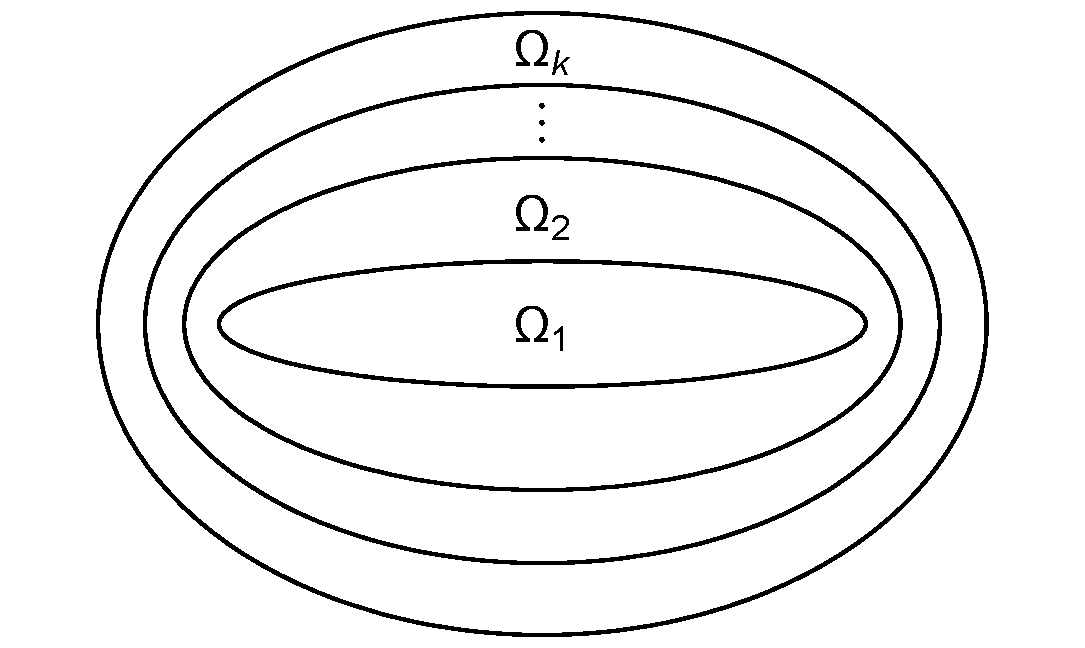
\includegraphics[width=0.35\linewidth]{images/ch3/multiple_ellipses.pdf}
        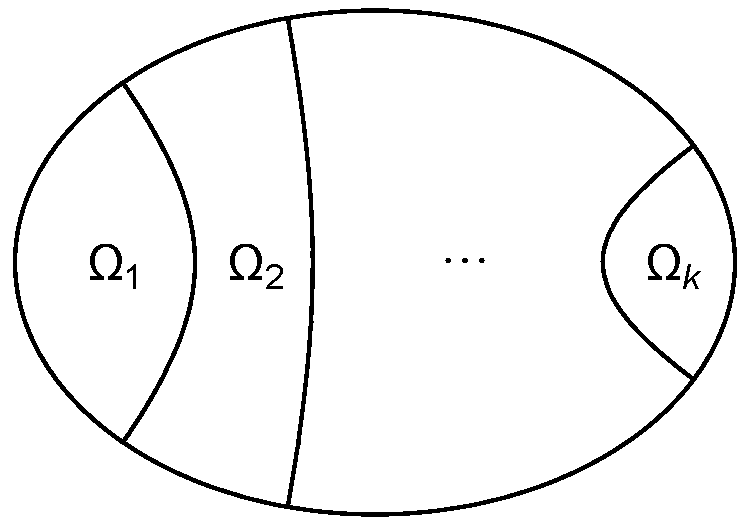
\includegraphics[width=0.29\linewidth]{images/ch3/multiple_hyperbolas.pdf}
    \end{minipage}
\caption{Взаимное расположение областей $\Omega_1, \ldots, \Omega_k$.}
\end{figure}

Здесь и далее коэффициент плотности в области $\Omega_j$ обозначим через $n_j$.

Определим функцию $\Xi(\mathbf{x}, \mathbf{v})$ по формуле: 
\begin{equation*}
\Xi(\mathbf{x}, \mathbf{v}) = \left[
\begin{array}{ll}
    \Lambda(\mathbf{x}, \mathbf{v}) n_1^2, &  \text{ если } \mathbf{x} \in \Omega_1 
    \\
    \Lambda(\mathbf{x}, \mathbf{v}) n_p^2 + 
    \sum_{j=1}^{p-1} \lambda_j(n_j^2-n_{j+1}^2), & \text{ если } \mathbf{x} \in \Omega_p \text{ для } 1 < p \leq k. 
\end{array}
\right.
\end{equation*}

\begin{theorem}
Функция $\Xi(\mathbf{x}, \mathbf{v})$ является константой на траекториях бильярда с модифицированным законом  преломления \eqref{eq:sect3_eq5}
\end{theorem}
Доказательство полностью аналогично доказательству теоремы из пункта 5.



\section{Преломление на пересекающихся софокусных квадриках.}

\subsection{ Случай 1: одна точка пересечения. }

Предположим, что внутренность эллипса разделена на области дугами софокусных квадрик таким образом, что имеются всего одна точка их пересечения, которую обозначим $A$.

Занумеруем области против часовой стрелки $\Omega_1, \Omega_2, \Omega_3, \Omega_4$. Пусть общая часть границы $\Omega_1 \cup \Omega_4$ и $\Omega_2 \cup \Omega_3$ --- дуга софокусной квадрики с параметром $\lambda_1$, а общая часть границы $\Omega_1 \cup \Omega_2$ и $\Omega_3 \cup \Omega_4$ --- дуга софокусной квадрики с параметром $\lambda_2$ (см. рис.2).

\begin{figure}[ht]
    \begin{minipage}[b][][b]{\linewidth}\centering
        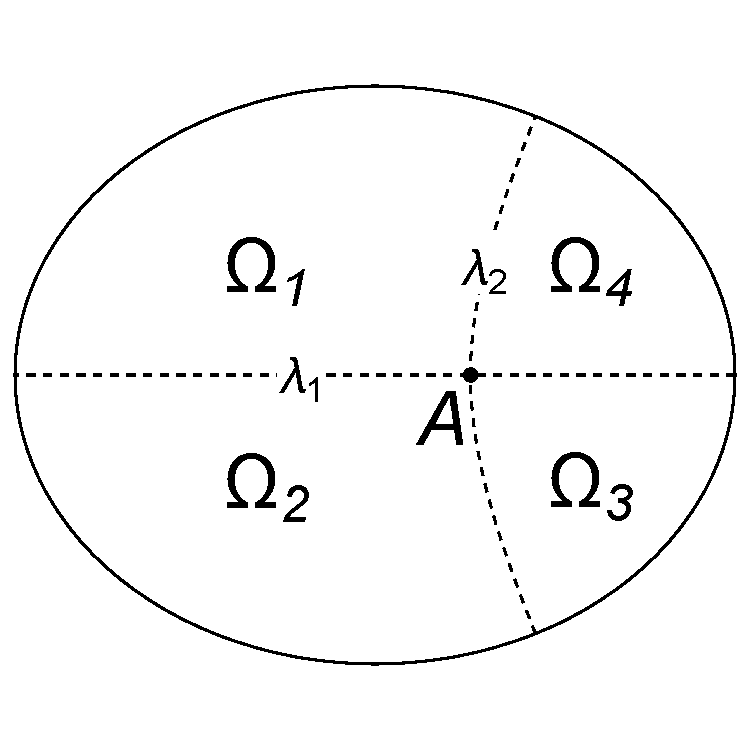
\includegraphics[width=0.35\textwidth]{images/ch3/img2.pdf}
    \end{minipage}
\caption{Взаимное расположение областей $\Omega_1,\ldots,\Omega_4$}
\end{figure}

Введем индекс ветвления в точке $A$ по формуле $$\gamma_A = \lambda_1(n_1^2 - n_2^2) + \lambda_2(n_2^2-n_3^2) + \lambda_1(n_3^2-n_4^2) + \lambda_2(n_4^2-n_1^2) = (\lambda_1 - \lambda_2) ( n_1^2 - n_2^2 + n_3^2 - n_4^2).$$

Определим в этой ситуации вспомогательную функцию $\widetilde{\Xi}(\mathbf{x}, \mathbf{v})$ 
\begin{equation*}
\widetilde{\Xi}(\mathbf{x}, \mathbf{v}) = \left[
\begin{array}{ll}
    \Lambda(\mathbf{x}, \mathbf{v}) n_1^2, &  \text{ если } \mathbf{x} \in \Omega_1 
    \\
    \Lambda(\mathbf{x}, \mathbf{v}) n_p^2 + 
    \sum_{j=1}^{p-1} \lambda_j(n_j^2-n_{j+1}^2), & \text{ если } \mathbf{x} \in \Omega_p \text{ для } 1 < p \leq 4. 
\end{array}
\right.
\end{equation*}
Неформально говоря, она почти подходит на роль дополнительного интеграла, но имеет разрыв на дуге, разделяющей области $\Omega_1$ и $\Omega_4$. Однако, как легко видеть, на любой бильярдной траектории, пересекающей эту дугу, она испытывает один и тот же скачок, равный индексу ветвления $\gamma_A$. 
Поэтому мы определим дополнительный интеграл $\Xi(\mathbf{x}, \mathbf{v})$ со значениями в $S^1= \mathbb{R}/\gamma_A \mathbb{Z}$ по формуле $$\Xi(\mathbf{x}, \mathbf{v}) = \widetilde{\Xi}(\mathbf{x}, \mathbf{v}) \mod \gamma_A.$$

Случай, когда границы раздела областей пересекаются по 2 и более точками сложнее. Мы приведем 2 примера, которые проиллюстрируют общую закономерность, заключающуюся в следующем: \\
\textit{ 
для каждой точки пересечения $A_i, i=1,\ldots,m$, определен индекс ветвления $\gamma_{A_i}$. Тогда дополнительный интеграл \  $\Xi(\mathbf{x}, \mathbf{v})$ принимает значения в $\mathbb{R}/(\gamma_{A_1} \mathbb{Z}+ \ldots + \gamma_{A_m} \mathbb{Z})$. Если $\gamma_{A_i}$ соизмеримы, т. е. всевозможные дроби $\dfrac{\gamma_{A_i}}{\gamma_{A_j}}$ --- рациональные числа (или бесконечность), то $\mathbb{R}/(\gamma_{A_1} \mathbb{Z}+ \ldots + \gamma_{A_m} \mathbb{Z}) = S^1$. Если же среди $\gamma_{A_i}$ есть пара с иррациональной дробью $\dfrac{\gamma_{A_i}}{\gamma_{A_j}}$, то подгруппа $\gamma_{A_1} \mathbb{Z}+ \ldots + \gamma_{A_m} \mathbb{Z}$ всюду плотна в $\mathbb{R}$. В этом случае, хотя дополнительный интеграл $\Xi(\mathbf{x}, \mathbf{v})$ корректно определен, но использовать его для топологического анализа структуры траекторий представляется весьма затруднительным.}

\bigskip
\subsection{ Случай 2: две точки пересечения.}

Рассмотрим области, изображенные на рис.3. 
\begin{figure}[ht]
\begin{minipage}{\linewidth}\centering
        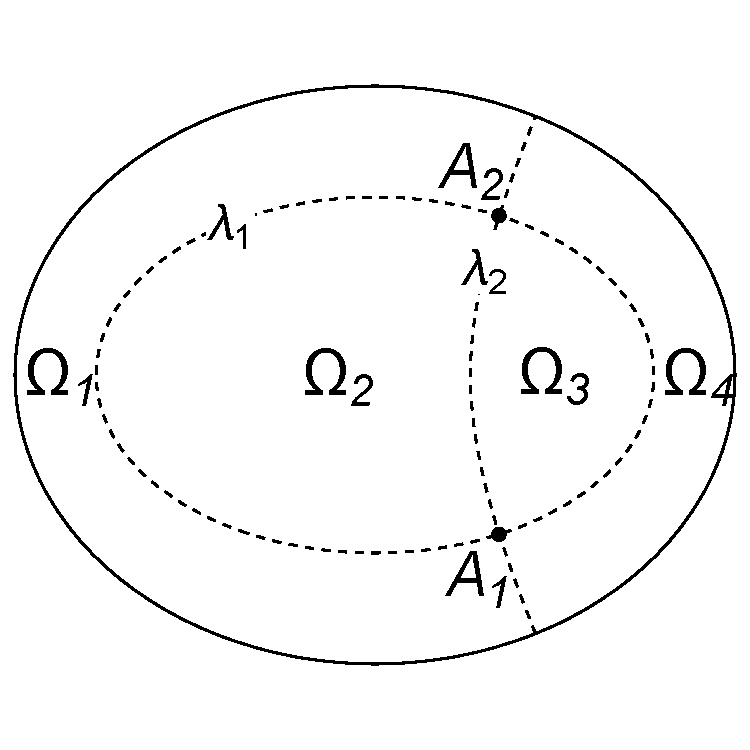
\includegraphics[width=0.35\linewidth]{images/ch3/img3.pdf}  
    \end{minipage}
\caption{Взаимное расположение областей $\Omega_1,\ldots,\Omega_4$}
\end{figure}


Легко вычислить индексы ветвления в точках $A_1, A_2$ (т.е. скачки дополнительного интеграла при обходе вокруг точки против часовой стрелки):
$$\gamma_{A_1} = \lambda_2(n_1^2 - n_4^2) + \lambda_1(n_4^2-n_3^2) + \lambda_2(n_3^2-n_2^2) + \lambda_1(n_2^2-n_4^2) = (\lambda_2 - \lambda_1) ( n_1^2 - n_2^2 + n_3^2 - n_4^2).$$
$$\gamma_{A_2} = \lambda_1(n_1^2 - n_2^2) + \lambda_2(n_2^2-n_3^2) + \lambda_1(n_3^2-n_4^2) + \lambda_2(n_4^2-n_1^2) = (\lambda_1 - \lambda_2) ( n_1^2 - n_2^2 + n_3^2 - n_4^2).$$
Как видно, в этом случае $$\gamma_{A_1} = -\gamma_{A_2}.$$
Поэтому дополнительный интеграл $\Xi(\mathbf{x}, \mathbf{v})$ может быть задан по модулю $\gamma_{A_1}$ формулой
\begin{equation*}
\Xi(\mathbf{x}, \mathbf{v}) = \left[
\begin{array}{ll}
    \Lambda(\mathbf{x}, \mathbf{v}) n_1^2, &  \text{ если } \mathbf{x} \in \Omega_1 
    \\
    \Lambda(\mathbf{x}, \mathbf{v}) n_p^2 + 
    \sum_{j=1}^{p-1} \lambda_j(n_j^2-n_{j+1}^2), & \text{ если } \mathbf{x} \in \Omega_p \text{ для } 1 < p \leq 4. 
\end{array}
\right.
\end{equation*}

\subsection{ Случай 3: две точки пересечения.}
Рассмотрим области, изображенные на рис.4. 

\begin{figure}[ht]
\begin{minipage}{\linewidth}\centering
        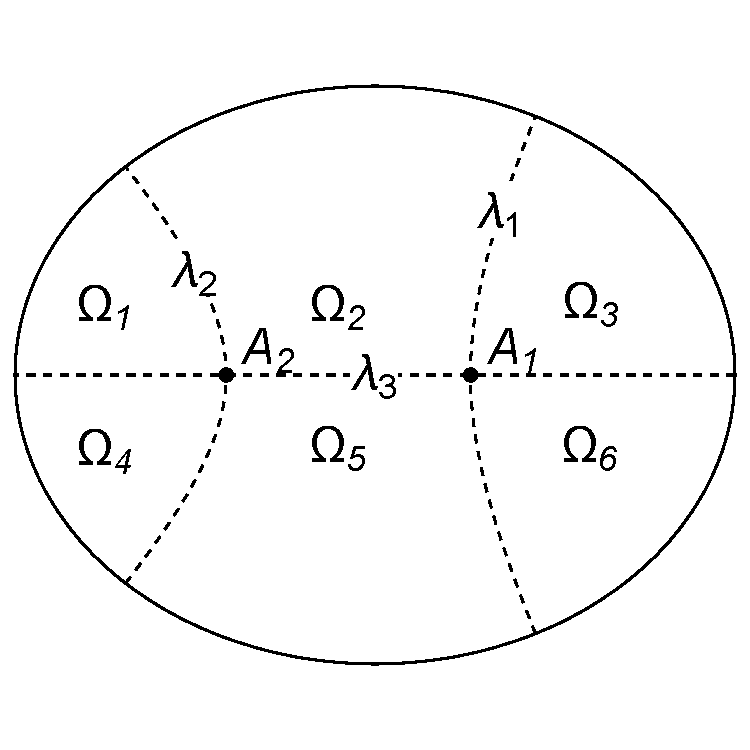
\includegraphics[width=0.25\linewidth]{images/ch3/img4.pdf}  
    \end{minipage}
\caption{Взаимное расположение областей $\Omega_1,\ldots,\Omega_6$}
\end{figure}

Легко видеть, что индексы ветвления в точках $A_1$, $A_2$ задаются формулами:
$$\gamma_{A_1} = (\lambda_3 - \lambda_1)(n_2^2 - n_5^2 + n_6^2 - n_3^2).$$
$$\gamma_{A_2} = (\lambda_3 - \lambda_2)(n_1^2 - n_4^2 + n_5^2 - n_2^2).$$

Ясно, что в зависимости от значений параметров отношение $\dfrac{\gamma_{A_1}}{\gamma_{A_2}}$ может быть как рациональным, так и иррациональным.
\bigskip


\clearpage
